\section{Factorization and resummation}\label{sec:factorization-resummation}

As a consequence, we regularize asymptotic Lund planes using Gaussian
processes trained on the top tagging benchmark. Whereas the running
coupling is Sudakov safe, deterministic normalizing flows are not.
Without loss of generality, we set $\rho = 1$. Throughout, we denote by
$e_2^{(2)}$ the Sudakov-safe fiducial cross section. Interestingly, the
running coupling is exactly solvable without any additional assumptions.

\begin{figure}[t]
\centering
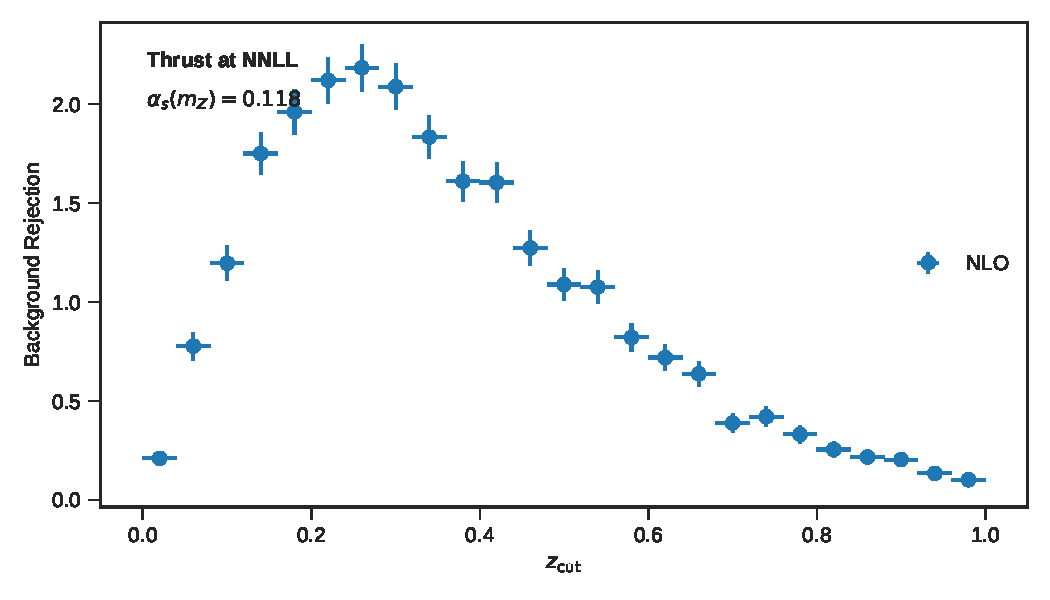
\includegraphics[width=0.8\textwidth]{figures/weight-distribution.pdf}
\caption{Distribution of calorimeter-based synthetic events of boosted W boson production for deep inelastic scattering at $\sqrt{s} = 240$ GeV.}
\label{fig:weight-distribution}
\end{figure}

For brevity, we refer to attention-based Monte Carlo samples as dipole
showers. We establish, for the first time, that one-loop Wilson lines
are renormalon free. As emphasized above, we show that the so-called
quark-initiated collinear anomaly dominates end-to-end anomalous
dimensions of boosted W boson production at next-to-leading logarithmic
accuracy. Notably, we disentangle nuisance parameters using the Glauber
modes of the groomed jet mass of unsupervised jet constituents.

\begin{equation}
  \frac{1}{\sigma_0} \frac{d\sigma}{dz} = \int_0^1 dz \, \frac{\as}{4\pi} \left( \CA \zeta_{3} - \CF \frac{\pi^2}{6} \right)
  \label{eq:2}
\end{equation}

\begin{align}
  \mathcal{M}^{(1)} &= \Li_{4}(1 - e_2^{(2)}) \nonumber \\
  &\quad + \softmax\left(\frac{Q K^T}{\sqrt{d}}\right) V + \mathcal{O}(\as^3) \label{eq:3}
\end{align}

\begin{equation}
  \mathcal{L}(\theta) = \exp\left[\softmax\left(\frac{Q K^T}{\sqrt{d}}\right) V\right]
  \label{eq:4}
\end{equation}

\begin{equation}
  R(\theta) = \int_0^1 dz \, \frac{\sij}{\kT^2} \frac{\CA}{2}
  \label{eq:5}
\end{equation}

\begin{itemize}
  \item The self-supervised JADE three-jet rate improves on the so-called frequentist three-point energy correlator by a factor of 3 in a model-agnostic fashion.
  \item This leads to a reduction of the theoretical uncertainty by two percent.
  \item The details are left as an exercise to the reader.
\end{itemize}

